\documentclass[10pt]{article}
\usepackage{tikz}
\usetikzlibrary{shapes.misc}
\usepackage[margin=0cm]{geometry}
\pagestyle{empty}
\tikzstyle{every node}=[cross out, draw, red]

\begin{document}

\vspace*{\fill}
\begin{center}
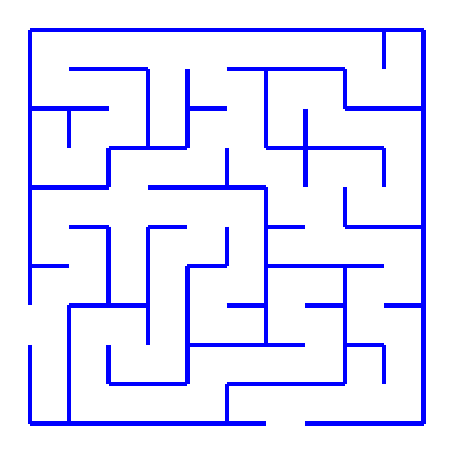
\begin{tikzpicture}[x=0.5cm, y=-0.5cm, ultra thick, blue]
% Walls
    \draw (0,0) -- (10,0);
    \draw (1,1) -- (3,1);
    \draw (5,1) -- (8,1);
    \draw (0,2) -- (2,2);
    \draw (4,2) -- (5,2);
    \draw (8,2) -- (10,2);
    \draw (2,3) -- (4,3);
    \draw (6,3) -- (9,3);
    \draw (0,4) -- (2,4);
    \draw (3,4) -- (6,4);
    \draw (1,5) -- (2,5);
    \draw (3,5) -- (4,5);
    \draw (6,5) -- (7,5);
    \draw (8,5) -- (10,5);
    \draw (0,6) -- (1,6);
    \draw (4,6) -- (5,6);
    \draw (6,6) -- (9,6);
    \draw (1,7) -- (3,7);
    \draw (5,7) -- (6,7);
    \draw (7,7) -- (8,7);
    \draw (9,7) -- (10,7);
    \draw (4,8) -- (7,8);
    \draw (8,8) -- (9,8);
    \draw (2,9) -- (4,9);
    \draw (5,9) -- (8,9);
    \draw (0,10) -- (6,10);
    \draw (7,10) -- (10,10);
    \draw (0,0) -- (0,7);
    \draw (0,8) -- (0,10);
    \draw (1,2) -- (1,3);
    \draw (1,7) -- (1,10);
    \draw (2,3) -- (2,4);
    \draw (2,5) -- (2,7);
    \draw (2,8) -- (2,9);
    \draw (3,1) -- (3,3);
    \draw (3,5) -- (3,8);
    \draw (4,1) -- (4,3);
    \draw (4,6) -- (4,9);
    \draw (5,3) -- (5,4);
    \draw (5,5) -- (5,6);
    \draw (5,9) -- (5,10);
    \draw (6,1) -- (6,3);
    \draw (6,4) -- (6,8);
    \draw (7,2) -- (7,4);
    \draw (8,1) -- (8,2);
    \draw (8,4) -- (8,5);
    \draw (8,6) -- (8,9);
    \draw (9,0) -- (9,1);
    \draw (9,3) -- (9,4);
    \draw (9,8) -- (9,9);
    \draw (10,0) -- (10,10);
% Pillars
% Inner points in accessible cul-de-sacs
% Entry-exit paths without intersections
\end{tikzpicture}
\end{center}
\vspace*{\fill}
\vspace*{\fill}

\end{document}
